\section{Contexte}

\subsection{Données}


Pour cette étude statistique et économétrique de la chirurgie ambulatoire dans les hôpitaux français, nous avons utilisé plusieurs bases de données en open access et mises à disposition par le gouvernement (Ministère de la santé ou Agence technique de l'information sur l'hospitalisation):

\begin{itemize}
    \item \textit{Open CCAM} (ATIH) de 2015 à 2019. Il s'agit de la base de données principale regroupant, pour chaque année, des informations sur les actes effectués dans chaque établissement de santé.
    \item \textit{Actes techniques CCAM} (CNAM) de 2015 à 2019. Cette base permet d'avoir accès à la tarification des actes.
    \item \textit{FINESS Extraction des établissements} (Ministère de la Santé) de 2015 à 2019. Cette base de données administrative donne des informations sur le statut des établissements de santé (Privé ou public).
    \item \textit{Hospidiag} ((ANAP, DGOS, HAS, IGAS, ATIH) de 2015 à 2019. La base de données est issue des enquêtes SAE (statistiques annuelles des établissements) et nous fournit des indicateurs sur les activités d'enseignement et de recherche ou sur la sévérité moyenne des cas traités par l'établissement.
\end{itemize}

\bigskip

Après fusion de ces bases de données, on obtient un tableau dans lequel une observation correspond au triplet (\textit{Acte CCAM}, \textit{Établissement}, \textit{Année}). Ainsi pour chaque année, on peut observer les informations sur les réalisations d'un acte CCAM par un établissement. Les variables les plus importantes, celles que nous allons utiliser, sont dans la base Open CCAM :

\begin{itemize}
    \item  Nombre de réalisation d'un acte (\textit{nb\_actes})
    \item Nombre de réalisation d'actes en ambulatoire (\textit{nb\_actes\_ambu})
    \item La durée moyenne de séjour (\textit{dms\_globale})
    \item Le nombre de séjour pour un acte (\textit{nb\_sejsea})
    \item Le nombre de séjour 0 nuit, correspondant aux séjours d'actes ambulatoires (\textit{nb\_sej\_0\_nuit}) 
\end{itemize}

\bigskip

La base de données Open CCAM a mis en place un système de censure, en effet, si un établissement réalise moins de 11 fois an un acte CCAM, alors celui-ci ne figure pas dans la base de données. De même si l'acte est réalisé moins de 11 fois en ambulatoire par l'établissement et par an, alors la donnée est censurée (elle est remplacée par un "."). Il en est de même pour les séjours.

\clearpage


\subsection{Répartition des hôpitaux}

On commence par regarder la répartition des établissements et des entités juridiques étudiés.\\

\begin{table}[ht]
\centering
\caption{Répartition des établissements de santé par année} 
\label{tri_eta}
\begin{tabular}{r|cccc|c}
  \hline
& Public & CHU & Privé lucratif & Privé non lucratif & Total\\ 
  \hline
2015 & 496 & 145 & 556 & 207 & 1404\\ 
  2016 & 576 & 142 & 492 & 196 & 1406 \\ 
  2017 & 582 & 143 & 498 & 207 & 1430 \\ 
  2018 & 573 & 144 & 503 & 216 & 1436\\ 
  2019 & 566 & 144 & 515 & 223 & 1448\\ 
   \hline
\end{tabular}
\end{table}

\bigskip

\begin{table}[ht]
\centering
\caption{Répartition des entités juridiques par année}
\label{tri_ej}
\begin{tabular}{r|cccc|c}
  \hline
 & Public & CHU & Privé lucratif & Privé non lucratif & Total \\ 
  \hline
2015 & 420 &  34 & 556 & 205 & 1215\\ 
  2016 & 490 &  31 & 492 & 196 & 1209\\ 
  2017 & 495 &  31 & 498 & 207 & 1231\\ 
  2018 & 486 &  31 & 503 & 216 & 1236\\ 
  2019 & 481 &  31 & 515 & 223 & 1250\\ 
   \hline
\end{tabular} 
\end{table}

\bigskip

On remarque qu'il y a 31 ou 34 entités juridiques au lieu de 30 pour les CHU, il s'agit du fait que différents établissements d'un même CHU portent des numéros FINESS (entité juridique) anormalement différents.\\


On peut également regarder la répartition géographique des établissements étudiés ainsi que l'évolution au cours du temps. Grâce au tableau \ref{tri_reg}, on constate que le nombre d'établissement varie très faiblement au cours du temps (Il en est de même pour les entités juridiques).

\clearpage



\begin{table}[!ht]
\centering
\caption{Répartition des établissements de santé par région} 
\label{tri_reg}
\begin{tabular}{l|ccccc}
  \hline
 & 2015 & 2016 & 2017 & 2018 & 2019 \\ 
  \hline
Auvergne-Rhône-Alpes & 152 & 159 & 164 & 161 & 162 \\ 
  Bourgogne-Franche-Comté &  62 &  64 &  65 &  61 &  59 \\ 
  Bretagne &  70 &  82 &  85 &  93 &  91 \\ 
  Centre-Val de Loire &  47 &  44 &  46 &  45 &  45 \\ 
  Corse &  10 &  12 &  11 &  10 &  10 \\ 
  Grand Est & 143 & 133 & 134 & 134 & 138 \\ 
  Guadeloupe, Martinique, Guyane &  28 &  24 &  23 &  26 &  26 \\ 
  Hauts-de-France & 126 & 126 & 128 & 124 & 123 \\ 
  Île-de-France & 219 & 200 & 209 & 210 & 211 \\ 
  Normandie &  74 &  74 &  73 &  73 &  74 \\ 
  Nouvelle-Aquitaine & 132 & 131 & 129 & 130 & 130 \\ 
  Occitanie & 121 & 134 & 134 & 138 & 138 \\ 
  Pays de la Loire &  69 &  75 &  83 &  83 &  84 \\ 
  Provence-Alpes-Côte d'Azur & 132 & 129 & 129 & 130 & 131 \\ 
  Réunion, Polynésie &  19 &  19 &  17 &  18 &  26 \\ 
   \hline
\end{tabular}
\end{table}

Les cartes \ref{carte_reg} et \ref{carte_dep} indiquent également des concentrations d'établissements assez conforme à la densité de population des départements ou régions. Les départements d'Outre-mer ne sont pas représentés sur ces cartes.\\

\begin{figure}[!hb]
    \centering
    \begin{minipage}{0.45 \linewidth}
    
        \centering
        \caption{Nombre d'établissements par région en 2019}
        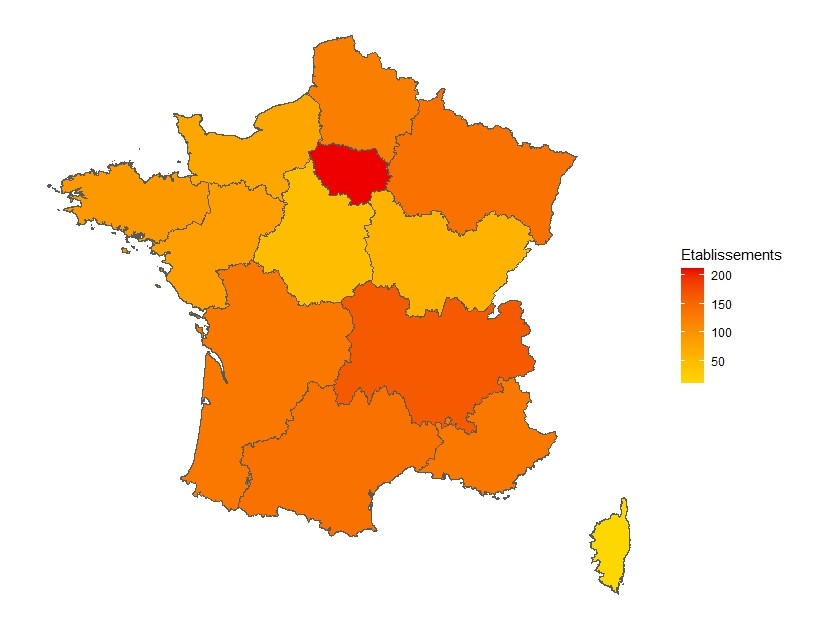
\includegraphics[width=1.1\linewidth]{Images/etablissement_reg_19.jpeg}
        \label{carte_reg}
    \end{minipage}
    \hfill
    \begin{minipage}{0.48 \linewidth}
        \centering
        \caption{Nombre d'établissements par département en 2019}
        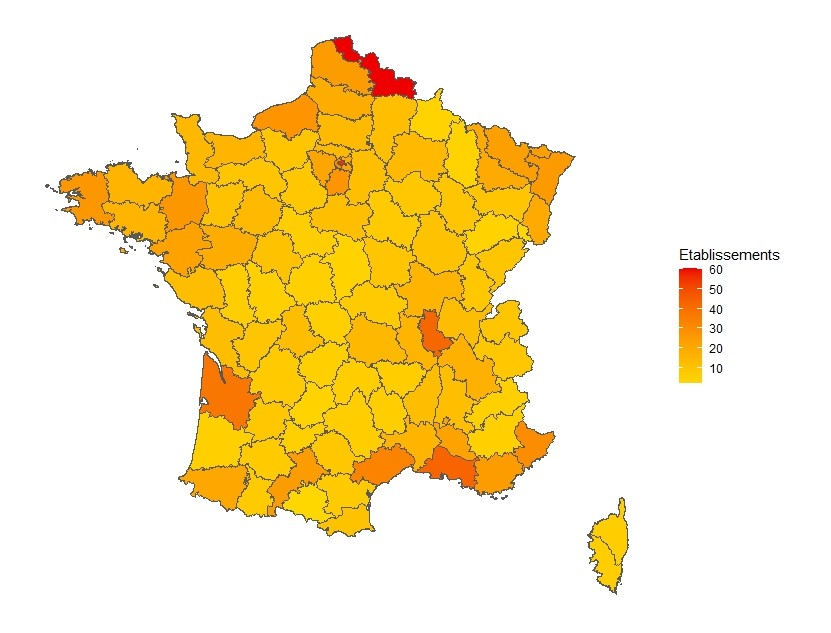
\includegraphics[width=1.1\linewidth]{Images/etablissement_dep_19.jpeg}
        \label{carte_dep}
    \end{minipage}
\end{figure}

\clearpage

Le tableau \ref{tri_cat_reg} présente la répartition des établissements par région et par catégorie \textit{CHU, Privé lucratif, Privé non lucratif} ou \textit{Public} ainsi que son évolution au cours des années. On peut ainsi observer comment les fermetures et ouvertures d'hôpitaux se répartissent entre les régions.\\


\begin{table}[hb]
\centering
\caption{Répartition des établissements de santé par région} 
\label{tri_cat_reg}
\scalebox{0.9}{
\begin{tabular}{l|c|cccc}
  \hline
Région & Année & CHU & Privé lucratif & Privé non lucratif & Public \\ 
  \hline
    \multirow{5}{*}{Auvergne-Rhône-Alpes} & 2015 &  21 &  55 &  17 &  59 \\ 
   & 2016 &  20 &  48 &  14 &  77 \\  
   & 2017 &  22 &  50 &  14 &  78 \\ 
   & 2018 &  22 &  51 &  14 &  74 \\ 
   & 2019 &  21 &  52 &  15 &  74 \\ 
   \hline
  \multirow{5}{*}{Bourgogne-Franche-Comté}    & 2015 &   4 &  19 &   3 &  36 \\ 
   & 2016 &   4 &  15 &   3 &  42 \\ 
   & 2017 &   3 &  16 &   3 &  43 \\ 
   & 2018 &   4 &  16 &   3 &  38 \\ 
   & 2019 &   4 &  16 &   3 &  36 \\ 
   \hline
  \multirow{5}{*}{Bretagne}    
  & 2015 &   7 &  14 &  22 &  27 \\ 
   & 2016 &   7 &  14 &  28 &  33 \\ 
   & 2017 &   8 &  14 &  29 &  34 \\ 
   & 2018 &   7 &  14 &  33 &  39 \\ 
   & 2019 &   8 &  16 &  33 &  34 \\ 
   \hline
  \multirow{5}{*}{Centre-Val de Loire}    & 2015 &   3 &  20 &   1 &  23 \\ 
   & 2016 &   3 &  15 &   1 &  25 \\ 
   & 2017 &   3 &  15 &   2 &  26 \\ 
   & 2018 &   3 &  15 &   2 &  25 \\ 
   & 2019 &   3 &  16 &   2 &  24 \\  
   \hline
  \multirow{5}{*}{Corse}    & 2015 &   0 &   4 &   0 &   6 \\ 
   & 2016 &   0 &   5 &   0 &   7 \\ 
   & 2017 &   0 &   5 &   0 &   6 \\ 
   & 2018 &   0 &   5 &   0 &   5 \\ 
   & 2019 &   0 &   5 &   0 &   5 \\ 
  \hline
  \multirow{5}{*}{Grand Est}    & 2015 &  13 &  29 &  42 &  59 \\ 
   & 2016 &  13 &  25 &  34 &  61 \\ 
   & 2017 &  13 &  25 &  35 &  61 \\ 
   & 2018 &  12 &  24 &  39 &  59 \\ 
   & 2019 &  13 &  25 &  41 &  59 \\
  \hline
  \multirow{5}{*}{Guadeloupe, Martinique, Guyane}    & 2015 &   6 &  13 &   2 &   7 \\ 
   & 2016 &   6 &  10 &   1 &   7 \\ 
   & 2017 &   5 &  10 &   1 &   7 \\ 
   & 2018 &   6 &  11 &   1 &   8 \\ 
   & 2019 &   6 &  11 &   1 &   8 \\ 
  \hline
\end{tabular}
}
\end{table}

\begin{table}[!t]
\centering
\scalebox{0.9}{
\begin{tabular}{l|c|cccc}
  \hline
Région & Année & CHU & Privé lucratif & Privé non lucratif & Public \\ 
  \hline
  \multirow{5}{*}{Hauts-de-France}    & 2015 &  11 &  52 &  12 &  51 \\ 
   & 2016 &  11 &  48 &  12 &  55 \\ 
   & 2017 &  11 &  49 &  12 &  56 \\ 
   & 2018 &  11 &  49 &  11 &  53 \\ 
   & 2019 &  10 &  48 &  12 &  53 \\  
  \hline
    \multirow{5}{*}{Île-de-France}    & 2015 &  33 & 109 &  34 &  43 \\ 
   & 2016 &  32 &  98 &  34 &  36 \\ 
   & 2017 &  33 &  99 &  34 &  43 \\ 
   & 2018 &  33 &  99 &  34 &  44 \\ 
   & 2019 &  31 &  99 &  35 &  46 \\ 
  \hline
\multirow{5}{*}{Normandie}    & 2015 &   5 &  26 &   7 &  36 \\ 
   & 2016 &   5 &  24 &   7 &  38 \\ 
   & 2017 &   5 &  24 &   6 &  38 \\ 
   & 2018 &   5 &  24 &   6 &  38 \\ 
   & 2019 &   5 &  24 &   7 &  38 \\ 
  \hline
  \multirow{5}{*}{Nouvelle-Aquitaine}    & 2015 &  11 &  57 &  16 &  48 \\ 
   & 2016 &   9 &  49 &  14 &  59 \\ 
   & 2017 &   9 &  49 &  14 &  57 \\ 
   & 2018 &   9 &  49 &  14 &  58 \\ 
   & 2019 &   9 &  51 &  14 &  56 \\
  \hline
  \multirow{5}{*}{Occitanie}    & 2015 &  12 &  57 &  11 &  41 \\ 
   & 2016 &  13 &  52 &  12 &  57 \\ 
   & 2017 &  13 &  54 &  11 &  56 \\ 
   & 2018 &  13 &  55 &  13 &  57 \\ 
   & 2019 &  14 &  54 &  13 &  57 \\  
  \hline
  \multirow{5}{*}{Pays de la Loire}    & 2015 &   4 &  27 &  14 &  24 \\ 
   & 2016 &   4 &  23 &  13 &  35 \\ 
   & 2017 &   5 &  22 &  22 &  34 \\ 
   & 2018 &   5 &  23 &  23 &  32 \\ 
   & 2019 &   5 &  23 &  23 &  33 \\ 
  \hline
  \multirow{5}{*}{Provence-Alpes-Côte d'Azur}    & 2015 &  10 &  62 &  26 &  34 \\ 
   & 2016 &  10 &  54 &  23 &  42 \\ 
   & 2017 &   9 &  55 &  24 &  41 \\ 
   & 2018 &  10 &  56 &  23 &  41 \\ 
   & 2019 &  10 &  56 &  24 &  41 \\  
   \hline
  \multirow{5}{*}{Réunion, Polynésie}    & 2015 &   5 &  12 &   0 &   2 \\ 
   & 2016 &   5 &  12 &   0 &   2 \\ 
   & 2017 &   4 &  11 &   0 &   2 \\ 
   & 2018 &   4 &  12 &   0 &   2 \\ 
   & 2019 &   5 &  19 &   0 &   2 \\ 
   \hline
\end{tabular}
}
\end{table}




\clearpage


\subsection{Actes les plus réalisés}

On regarde ici les actes les plus réalisés, globalement puis par catégories.


\begin{table}[!ht]
\centering
\caption{Liste des 20 actes les plus réalisés entre 2015 et 2019} 
\begin{tabular}{c|cl}
  \hline
Code CCAM & Fréquence & Libellé abrégé de l'acte \\ 
  \hline
ZBQK0020 & 5.78 \% & Radiographie du thorax \\ 
  DEQP0030 & 4.81 \% & Électrocardiographie sur au moins 12 dérivations \\ 
  DEQP0070 & 4.54 \% & Surveillance continue de l'électrocardiogramme par oscilloscopie\\ 
  JVJF0040 & 3.45 \% & Séance d'épuration extrarénale par hémodialyse \\ 
  YYYY6000 & 3.31 \% & Supplément pour archivage numérique d'une mammographie \\ 
  ZZLP0250 & 3.04 \% & Anesthésie générale ou locorégionale complémentaire niveau 1 \\ 
  JVJF0080 & 1.84 \% & Séance d'épuration extrarénale par hémodiafiltration\\ 
  GLLD0170 & 1.77 \% & Oxygénothérapie avec surveillance continue de l'oxymétrie \\ 
  YYYY0150 & 1.72 \% & Forfait de réanimation niveau A \\ 
  HEQE0020 & 1.45 \% & Endoscopie oeso-gastro-duodénale \\ 
  GLHF0010 & 1.11 \% & Prélèvement de sang artériel (gazométrie sanguine, mesure du pH) \\ 
  EQQP0110 & 1.1 \% & Surveillance continue de la pression intraartérielle \\ 
  DZQM0060 & 1.06 \% & Échographie-doppler transthoracique du coeur \\ 
  ACQK0010 & 1.04 \% & Scanographie du crâne et de son contenu \\ 
  DEQP0040 & 1 \% & Surveillance continue de l'électrocardiogramme par oscilloscopie \\ 
  BFGA0040 & 0.95 \% & Extraction du cristallin avec implantation de cristallin artificiel \\ 
  ZZQP0040 & 0.86 \% & Restitution tridimensionnelle des images acquises par scanographie \\ 
  FELF0110 & 0.84 \% & Transfusion de concentré de globules rouges \\ 
  GELD0050 & 0.84 \% & Nébulisation d'agent thérapeutique à destination bronchique \\ 
  ZZNL0630 & 0.83 \% & Séance d'irradiation externe par accélérateur linéaire  (5MV) \\ 
   \hline
\end{tabular}
\end{table}



\begin{table}[!ht]
\centering
\caption{Liste des 10 premières catégories d'actes les plus réalisés}
\begin{tabular}{l|cc}
  \hline
Catégorie d'acte & Nombre d'actes & Fréquence \\ 
  \hline
Actes techniques médicaux thérapeutiques & 93753918 & 28.66 \% \\ 
  Actes techniques médicaux diagnostiques & 75446683 & 23.06 \% \\ 
  Imagerie Radiographie & 42860943 & 13.1 \% \\ 
  Actes chirurgicaux & 38700959 & 11.83 \% \\ 
  Imagerie Échographie & 17727895 & 5.42 \% \\ 
  Imagerie Scanographie & 15399861 & 4.71 \% \\ 
  Accouchements et actes obstétricaux & 9392094 & 2.87 \% \\ 
  Examen immunologique de prélèvement cellulaire ou tissulaire & 4798810 & 1.47 \% \\ 
  Autres Actes Médicaux Thérapeutiques & 4186869 & 1.28 \% \\ 
  Autres examens de matériel d'exérèse non à visée carcinologique & 3422644 & 1.05 \% \\ 
   \hline
\end{tabular}
\end{table}


On va donc s'intéresser aux actes des 4 catégories les plus importantes, concentrant chacune au moins 10\% des actes. Pour chacune d'entre elles, on va regarder les actes les plus réalisés, leur fréquence au sein de la catégorie ainsi que leur part d'actes en ambulatoire. Voir tableaux \ref{liste1}, \ref{liste2}, \ref{liste3} et \ref{liste4}.

\`{A} noter que la donnée "nombre d'actes en ambulatoire" est indisponible pour les années de 2015 à 2017. On va donc approcher cette donnée par le "nombre de séjour de 0 nuit". Cette approximation sera étudiée plus en détails dans la section \ref{Approx}.\\


\begin{table}[!ht]
\centering
\caption{Liste des actes techniques médicaux thérapeutiques les plus réalisés}
\label{liste1}
\begin{tabular}{c|ccl}
  \hline
Code CCAM & Fréquence & Ambulatoire & Libellé abrégé de l'acte \\ 
  \hline
JVJF0040 & 13.57 \% & 93.88 \% & Séance d'épuration extrarénale par hémodialyse\\ 
  JVJF0080 & 7.23 \% & 96.91 \% & Séance d'épuration extrarénale par hémodiafiltration \\ 
  GLLD0170 & 6.98 \% & 2.08 \% & Oxygénothérapie avec surveillance continue de l'oxymétrie \\ 
  YYYY0150 & 6.79 \% & 0.16 \% & Forfait de réanimation niveau A \\ 
  FELF0110 & 3.31 \% & 24.75 \% & Transfusion de concentré de globules rouges \\ 
  GELD0050 & 3.29 \% & 1.57 \% & Nébulisation d'agent thérapeutique à destination bronchique \\ 
  ZZNL0630 & 3.29 \% & 95.09 \% & Séance d'irradiation externe (Puissance de 5 MV) \\ 
  GLLD0150 & 3.08 \% & 0.55 \% & Ventilation mécanique intratrachéale \\ 
  BELB0010 & 2.86 \% & 92.92 \% & Injection de substance dans la chambre antérieure de l'oeil \\ 
  YYYY0200 & 2.53 \% & 0.35 \% & Forfait de réanimation niveau B \\ 
  HSLD0010 & 2.37 \% & 0.09 \% & Alimentation entérale par sonde (20 à 35 kcal/kg/jour) \\ 
  ZZNL0540 & 2.28 \% & 95.38 \% & Séance d'irradiation externe par accélérateur linéaire \\ 
  HSLD0020 & 2.19 \% & 0.1 \% & Alimentation entérale par sonde (plus de 35 kcal/kg/jour) \\ 
  GLLD0080 & 1.9 \% & 0.63 \% & Ventilation mécanique intratrachéale \\ 
  GLLD0030 & 1.85 \% & 0.2 \% & Ventilation spontanée au masque facial, par canule nasale \\ 
   \hline
\end{tabular} 
\end{table}



\begin{table}[!b]
\centering
\caption{Liste des actes techniques médicaux diagnostiques les plus réalisés} 
\label{liste2}
\begin{tabular}{c|ccl}
  \hline
Code CCAM & Fréquence & Ambulatoire & Libellé abrégé de l'acte \\ 
  \hline
DEQP0030 & 23.54 \% & 12.13 \% & Électrocardiographie sur au moins 12 dérivations \\ 
  DEQP0070 & 22.22 \% & 2.78 \% & Surveillance de l'électrocardiogramme, pression intraartérielle\\ 
  HEQE0020 & 7.11 \% & 73.37 \% & Endoscopie oeso-gastro-duodénale \\ 
  GLHF0010 & 5.43 \% & 4.31 \% & Prélèvement de sang artériel (gazométrie, mesure du pH) \\ 
  EQQP0110 & 5.35 \% & 0.41 \% & Surveillance continue de la pression intraartérielle \\ 
  DEQP0040 & 4.89 \% & 3.28 \% & Surveillance continue de l'électrocardiogramme \\ 
  HHQE0050 & 3.73 \% & 86.03 \% & Coloscopie totale avec visualisation du bas-fond caecal \\ 
  GLQP0050 & 2.1 \% & 1.32 \% & Enregistrement continu de la saturation sanguine en oxygène \\ 
  HHQE0020 & 1.75 \% & 87.65 \% & Coloscopie totale avec franchissement de l'orifice iléocolique \\ 
  GLQP0020 & 1.14 \% & 31.78 \% & Mesure de la capacité vitale lente et de l'expiration forcée \\ 
  DEQP0050 & 1.05 \% & 4.05 \% & Électrocardiographie sur au moins 2 dérivations \\ 
  ENLF0010 & 0.76 \% & 0.96 \% & Pose de dispositif de surveillance de la pression intraartérielle \\ 
  CDQP0090 & 0.75 \% & 0.19 \% & Enregistrement des otoémissions \\ 
  AAQP0070 & 0.6 \% & 7.8 \% & Électroencéphalographie sur 8 dérivations ou plus \\ 
  FEHB0010 & 0.57 \% & 2.39 \% & Prélèvement de sang artériel, par voie transcutanée \\ 
   \hline
\end{tabular}
\end{table}



\begin{table}[!ht]
\centering
\caption{Liste des actes d'imagerie et radiographie les plus réalisés}
\label{liste3}
\begin{tabular}{c|ccl}
  \hline
Code CCAM & Fréquence & Ambulatoire & Libellé abrégé de l'acte \\ 
  \hline
ZBQK0020 & 49.72 \% & 8.13 \% & Radiographie du thorax \\ 
  ZZQP0040 & 7.4 \% & 10.01 \% & Restitution tridimensionnelle des images (scanographie) \\ 
  ZZQK0020 & 4.88 \% & 2.37 \% & Radiographie au lit du malade (1 ou 2 incidences) \\ 
  ZCQK0020 & 4.12 \% & 8.86 \% & Radiographie de l'abdomen sans préparation \\ 
  NFQK0010 & 3.05 \% & 8.26 \% & Radiographie unilatérale du genou (1 ou 2 incidences) \\ 
  NAQK0150 & 2.65 \% & 8.12 \% & Radiographie de la ceinture pelvienne (1 incidence) \\ 
  NEQK0100 & 2.33 \% & 1.92 \% & Radiographie de l'articulation coxofémorale \\ 
  MAQK0030 & 1.99 \% & 11.42 \% & Radiographie de la ceinture scapulaire/épaule \\ 
  ZZQN0020 & 1.69 \% & 18.12 \% & Restitution tridimensionnelle des images (IRM) \\ 
  NAQK0710 & 1.67 \% & 2.67 \% & Radiographie unilatérale de l'articulation coxofémorale \\ 
  NDQK0010 & 1.45 \% & 25.77 \% & Radiographie unilatérale du pied (1 à 3 incidences) \\ 
  MGQK0030 & 1.43 \% & 18.15 \% & Radiographie du poignet (1 ou 2 incidences) \\ 
  NGQK0010 & 1.33 \% & 11.09 \% & Radiographie de la cheville (1 à 3 incidences) \\ 
  MDQK0010 & 1.25 \% & 36.87 \% & Radiographie de la main ou de doigt \\ 
  LFQK0020 & 1.17 \% & 8.36 \% & Radiographie de la colonne vertébrale (1 à 3 incidences) \\ 
   \hline
\end{tabular}
\end{table}


\begin{table}[!b]
\centering
\caption{Liste des actes chirurgicaux les plus réalisés} 
\label{liste4}
\begin{tabular}{c|ccl}
  \hline
Code CCAM & Fréquence & Ambulatoire & Libellé abrégé de l'acte \\ 
  \hline
BFGA0040 & 9.07 \% & 93.31 \% & Extraction du cristallin avec implantation de cristallin artificiel \\ 
  HZHE0020 & 5.72 \% & 72.34 \% & Biopsie et/ou brossage cytologique de la paroi du tube digestif \\ 
  HHFE0020 & 4.69 \% & 89.68 \% & Exérèse de polypes de moins de 1cm de diamètre du côlon \\ 
  EPLF0020 & 2.62 \% & 5.6 \% & Pose d'un cathéter veineux central, par voie transcutanée \\ 
  EBLA0030 & 2.14 \% & 60.14 \% & Pose d'un cathéter sur une veine profonde du membre supérieur\\ 
  HMFC0040 & 1.46 \% & 35.61 \% & Cholécystectomie, par coelioscopie \\ 
  BFGA4270 & 1.4 \% & 95.59 \% & Extraction, implantation de cristallin sans drainage trabéculaire\\ 
  HHFE0060 & 1.18 \% & 79.04 \% & Séance de mucosectomie rectocolique, par endoscopie \\ 
  AHPA0090 & 1.14 \% & 93.41 \% & Libération du nerf médian au canal carpien, par abord direct \\ 
  JHFA0090 & 1.1 \% & 94.31 \% & Posthectomie \\ 
  PAGA0110 & 1.07 \% & 72 \% & Ablation de matériel d'ostéosynthèse des membres sur un site \\ 
  JCLE0020 & 1.03 \% & 22.15 \% & Pose d'une endoprothèse urétérale, par endoscopie rétrograde \\ 
  NEKA0200 & 1.02 \% & 0.83 \% & Remplacement de l'articulation coxofémorale par prothèse \\ 
  NFFC0040 & 0.99 \% & 90.61 \% & Méniscectomie latérale ou médiale du genou, par arthroscopie \\ 
  HHFE0040 & 0.86 \% & 83.32 \% & Exérèse de polypes de plus de 1cm de diamètre du côlon \\ 
  QZMA0010 & 0.85 \% & 68.38 \% & Réparation de perte de substance par lambeau local ou régional \\ 
  JJFJ0010 & 0.82 \% & 98.3 \% & Prélèvement d'ovocytes sur un ou deux ovaires \\ 
  LMMA0120 & 0.8 \% & 61.5 \% & Cure unilatérale d'une hernie de l'aine avec pose de prothèse \\ 
  QCJA0010 & 0.77 \% & 77.92 \% & Parage et/ou suture de plaie profonde de la main \\ 
  EJGA0020 & 0.69 \% & 77.06 \% & Extraction de la grande veine saphène, par abord direct \\ 
   \hline
\end{tabular}
\end{table}

\newpage


Nous allons donc nous concentrer sur les actes pour lesquels le taux d'ambulatoire n'est ni trop haut ni trop bas (intervalle déterminé dans la sous-partie \ref{intervalle}) afin de mettre plus en valeur les différences au travers des années et entre les hôpitaux. Les actes chirurgicaux respectent plutôt bien cette condition, on s'intéressera tout de même à certains actes médicaux et d'imageries. 


\subsection{\'{E}tude du taux d'ambulatoire et du nombre d'actes} \label{intervalle}


Dans cette sous-partie nous allons étudier la distribution du taux d'actes en ambulatoire et du nombre d'actes (agrégation par acte CCAM). Cela va permettre de trouver des intervalles optimaux pour sélectionner les actes ou regroupement d'actes les plus pertinents à étudier. Cette sélection est nécessaire pour l'analyse globale des actes car la taille de la base de données initiale est trop importante et induit des problèmes de puissance de calcul. Ici, une observation correspond donc à un acte CCAM et le nombre d'actes associé correspond au nombre total de fois qu'il a été réalisé (de 2015 à 2019 et dans tous les établissements).


\begin{table}[ht]
\centering
\caption{Descriptif du taux d'actes en ambulatoire} 
\begin{tabular}{cccccc}
  \hline
Min. & 1er Qu. & Médiane & Moyenne & 3e Qu. & Max. \\ 
  \hline
0.00 & 0.00 & 7.73 & 25.60 & 48.09 & 100.00 \\ 
   \hline
\end{tabular}
\end{table}



\begin{figure}[!ht]
    \centering
    \caption{Histogramme du taux d'actes en ambulatoire}
    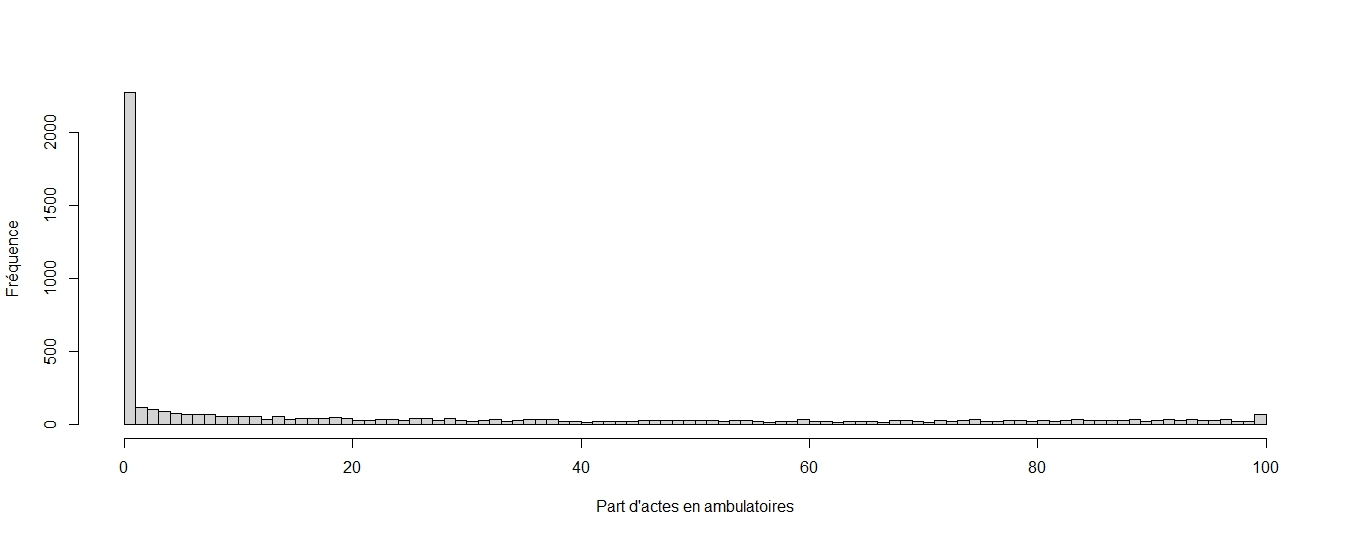
\includegraphics[scale=0.55]{Images/hist_part_ambu.jpeg}
    \label{hist_part_ambu}
\end{figure}

On observe que de nombreux actes ont un taux de 0, plus précisément, \textbf{36.1\% des actes ne sont jamais réalisés en ambulatoires}. Puisque ces actes ne nous intéressent pas pour cette étude, nous nous concentrons dans cette sous-partie uniquement sur les actes réalisables en ambulatoire.\\


\begin{table}[!ht]
\centering
\caption{Descriptif du taux d'actes en ambulatoire\\(Actes réalisables en ambulatoire)} 
\label{stat_part_AReA}
\begin{tabular}{cccccc}
  \hline
Min. & 1st Qu. & Median & Mean & 3rd Qu. & Max. \\ 
  \hline
0.02 & 9.91 & 33.08 & 40.09 & 68.97 & 100.00 \\  
   \hline
\end{tabular}
\end{table}

\bigskip


\begin{figure}[!ht]
    \centering
    \caption{Histogramme du taux d'actes en ambulatoire \\(Actes réalisables en ambulatoire)}
    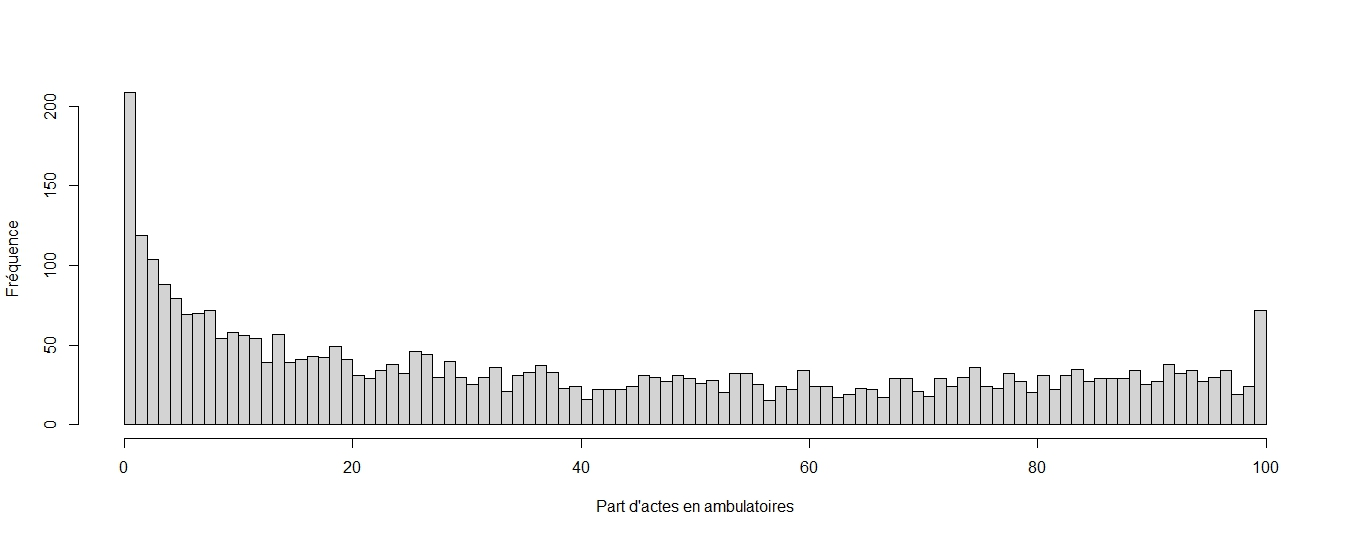
\includegraphics[scale=0.5]{Images/hist_part_ambu_non_nul.jpeg}
    \label{hist_part_ambu_non_nul}
\end{figure}

Grâce aux statistiques du tableau \ref{stat_part_AReA} et l'histogramme \ref{hist_part_ambu_non_nul}, on remarque désormais que la distribution du taux d'actes en ambulatoire est plutôt uniforme, en particulier pour des taux supérieurs à 20\%. Avant de fixer un intervalle sur le taux d'actes en ambulatoire, nous allons également étudier la distribution du nombre d'actes afin de fixer également un intervalle de sélection sur cette variable.\\



\begin{table}[!ht]
\centering
\caption{Descriptif du nombre d'actes\\(Actes réalisables en ambulatoires)} 
\begin{tabular}{cccccc}
  \hline
Min. & 1st Qu. & Median & Mean & 3rd Qu. & Max. \\ 
  \hline
11.00 & 693.50 & 4026.00 & 99068.87 & 23984.00 & 21311816.00 \\ 
   \hline
\end{tabular}
\end{table}



On observe que la moyenne est sensiblement différente de la médiane, cela est dû à la présence de valeurs extrêmes. En effet, la valeur maximale est bien plus élevée que le troisième quartile voire même du \textbf{quantile d'ordre 95 qui est à 262234} contre 21311816 pour le maximum. On choisit donc de passer le nombre d'actes au logarithme décimal afin de rendre la donnée plus exploitable comme on peut le constater avec l'histogramme \ref{log_nb_actes} et le tableau \ref{log_stat_nb}, ce dernier nous montre en effet que les statistiques sont bien plus régulières, on allons donc préférer étudier le logarithme du nombre d'actes réalisés.


\begin{table}[!ht]
\centering
\caption{Descriptif du logarithme du nombre d'actes\\(Actes réalisables en ambulatoires)} 
\label{log_stat_nb}
\begin{tabular}{cccccc}
  \hline
Min. & 1st Qu. & Median & Mean & 3rd Qu. & Max. \\ 
  \hline
2.40 & 6.54 & 8.30 & 8.30 & 10.09 & 16.87 \\ 
   \hline
\end{tabular}
\end{table}



\begin{figure}[!ht]
    \centering
    \caption{Histogramme du logarithme du nombre d'actes\\(Actes réalisables en ambulatoire)}
    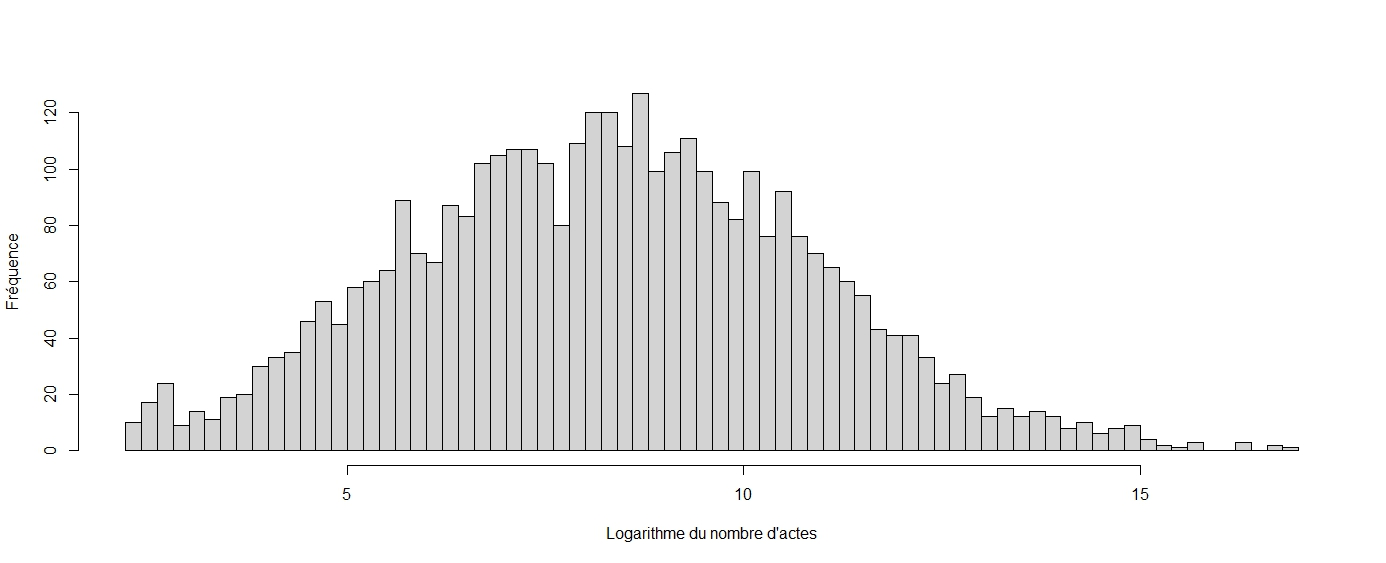
\includegraphics[scale=0.55]{Images/log_nb_actes.jpeg}
    \label{log_nb_actes}
\end{figure}

La figure \ref{nuage_part_nb}, ci-dessous, représente chaque acte CCAM selon son taux d'ambulatoire en abscisse, et le nombre de fois qu'il a été réalisé en ordonnée. Grâce à l'amas de points à gauche, on constate déjà que de nombreux actes sont rarement réalisées en ambulatoire. On observe également une minoration par le bas pour les actes réalisés peu de fois et ayant un faible taux d'ambulatoire, c'est-à-dire que les actes qui sont réalisés peu de fois en ambulatoire ont tendance à être des actes assez communs. Les actes avec un très fort taux d'ambulatoire sont, par ailleurs, des actes réalisés peu de fois (ligne verticale en bas à droite).


Outre ces détails et passé le taux d'actes en ambulatoire de 15\%, le nuage de points parait plutôt uniforme. Afin d'avoir assez d'actes à étudier, nous allons garder ceux pour lesquels le \textbf{taux d'ambulatoire est situé entre 15 et 85\%}, nous nous concentrerons également que sur les actes réalisés de nombreuses fois, c'est-à-dire \textbf{plus de 5000 fois} ($log 
5000 \approx 8.5$). On obtient donc l'encadrement visible sur la figure \ref{nuage_part_nb}, on sélectionne ainsi \textbf{848 actes distincts, c'est-à-dire 14.8\% des actes}. Ces intervalles ont également été choisis pour maximiser le R\up{2} ajusté de la régression de base dont la formule est donnée par l'équation \ref{eqn:equation_base}, le R\up{2} ajusté obtenu est de 20.01\%.\\


 


\begin{figure}[!ht]
    \centering
    \caption{Actes selon leur quantité et leur taux d'ambulatoire\\(Actes réalisables en ambulatoire)}
    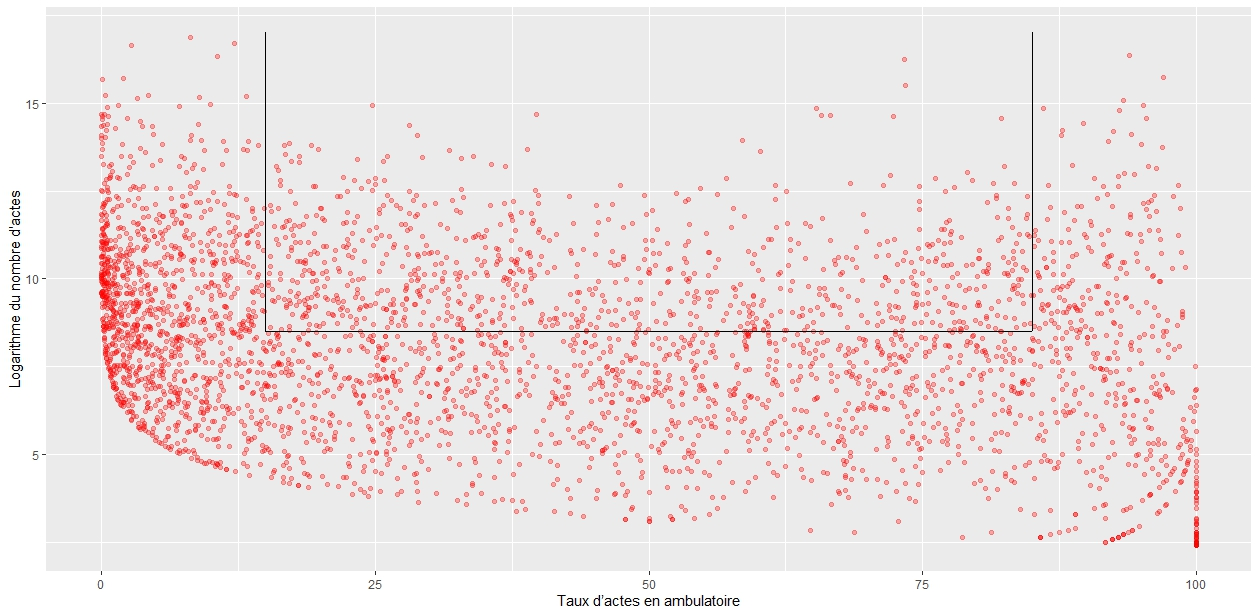
\includegraphics[scale=0.55]{Images/nuage_part_nb.jpeg}
    \label{nuage_part_nb}
\end{figure}


On peut désormais étudier de nouveau quels sont les actes les plus fréquents, de manière générale puis par catégorie afin de savoir lesquels seraient pertinents à analyser individuellement. 

Le tableau \ref{cat_select} présente les catégories d'actes sélectionnés les plus réalisés, c'est-à-dire avec une fréquence supérieure à 5\%. On remarque que parmi les actes sélectionnés, ce sont les actes chirurgicaux qui sont les plus nombreux, ce qui reste conforme à l'intuition précédente, l'analyse de la médecine ambulatoire à l'air assez pertinente lorsqu'on se concentre sur la chirurgie. Dans la suite de cette partie, on va se concentrer seulement sur les 4 premières catégories ainsi que sur les actes les plus réalisés.\\

\begin{table}[!ht]
\centering
\caption{Catégories les plus importantes des actes sélectionnés} 
\label{cat_select}
\begin{tabular}{l|ccc}
  \hline
Catégorie d'acte & Nombre d'actes & Fréquence & Actes distincts \\ 
  \hline
Actes chirurgicaux & 16871438 & 23.01 \% & 327 \\ 
  Actes techniques médicaux diagnostiques & 14698791 & 20.05 \% & 152 \\ 
  Actes techniques médicaux thérapeutiques & 10066498 & 13.73 \% & 132 \\ 
  Examen immunologique de prélèvement cellulaire/tissulaire & 4798810 & 6.54 \% &   9 \\ 
  Imagerie Échographie & 4653937 & 6.35 \% &  45 \\ 
  Imagerie Radiographie & 3740717 & 5.1 \% &  30 \\  
   \hline
\end{tabular}
\end{table}


\begin{table}[!ht]
\centering
\caption{Liste des 10 actes sélectionnés les plus réalisés} 
\label{actes_select}
\begin{tabular}{ccl}
  \hline
Acte CCAM & Fréquence & Catégorie d'acte \\ 
  \hline
ZZLP0250 & 3.04 \% &  \\ 
  HEQE0020 & 1.45 \% & Actes techniques médicaux diagnostiques \\ 
  FELF0110 & 0.84 \% & Actes techniques médicaux thérapeutiques \\ 
  AHQJ0210 & 0.76 \% &  \\ 
  ZZQX1880 & 0.65 \% & Autres examens de matériel d'exérèse non à visée carcinologique \\ 
  ZZQX1620 & 0.63 \% & Autres examens de biopsie \\ 
  ZZQX0690 & 0.62 \% & Examen immunologique de prélèvement cellulaire ou tissulaire \\ 
  HZHE0020 & 0.6 \% & Actes chirurgicaux \\ 
  ZZQX0770 & 0.58 \% & Examen de biopsie étagée \\ 
  YYYY0120 & 0.48 \% &  \\ 
   \hline
\end{tabular}
\end{table}



Grâce au tableau \ref{actes_select}, on constate que parmi les actes les plus réalisés, certains n'ont pas de catégorie renseignée. Ce sont des actes d'anesthésie ou des actes supplémentaires, ils sont effectués en complément d'actes chirurgicaux pouvant être de nature très différente, ils sont donc trop généraux pour être étudiés individuellement, ils ne permettent pas de passer outre la sélection des cas moins complexes par les hôpitaux privés.

\begin{itemize}
    \item ZZLP0250 : Anesthésie générale ou locorégionale complémentaire niveau 1

    \item AHQJ0210 : Guidage échographique pour anesthésie locorégionale périphérique du cou, du sein, de la paroi thoracique, de la paroi abdominale ou de membre, ou pour anesthésie rachidienne des patients dont l'indice de masse corporelle est supérieur ou égal à 30 kg/m2

    \item YYYY0120 : Supplément pour radiographie per opératoire au cours d'un acte de chirurgie orthopédique ou traumatologique
    
\end{itemize}

\bigskip


\begin{table}[!ht]
    \centering
    \begin{minipage}[t]{0.45 \linewidth}
  
\caption{Liste 10 actes les plus effectués en chirurgie} 
\label{actes_chiru}
\begin{tabular}{lcc}
  \hline
Acte CCAM & Nombre d'actes & Fréquence \\ 
  \hline
HZHE0020 & 2213489 & 0.6 \% \\ 
  EBLA0030 & 828022 & 0.22 \% \\ 
  HMFC0040 & 563437 & 0.15 \% \\ 
  HHFE0060 & 457461 & 0.12 \% \\ 
  PAGA0110 & 415093 & 0.11 \% \\ 
  JCLE0020 & 398527 & 0.11 \% \\ 
  HHFE0040 & 333227 & 0.09 \% \\ 
  QZMA0010 & 328763 & 0.09 \% \\ 
  LMMA0120 & 310259 & 0.08 \% \\ 
  QCJA0010 & 298811 & 0.08 \% \\ 
   \hline
\end{tabular}

\end{minipage}
\hfill
\begin{minipage}[t]{0.48 \linewidth}

\centering
\caption{Liste 10 actes les plus effectués en médecine diagnostique} 
\label{actes_diag}
\begin{tabular}{lcc}
  \hline
Acte CCAM & Nombre d'actes & Fréquence \\ 
  \hline
HEQE0020 & 5366259 & 1.45 \% \\ 
  GLQP0020 & 861763 & 0.23 \% \\ 
  ALQP0060 & 382192 & 0.1 \% \\ 
  GEQE0070 & 365411 & 0.1 \% \\ 
  EQQM0060 & 347233 & 0.09 \% \\ 
  GLQP0120 & 317504 & 0.09 \% \\ 
  HMQJ0010 & 289671 & 0.08 \% \\ 
  HJQE0010 & 286504 & 0.08 \% \\ 
  BGQP0020 & 277148 & 0.08 \% \\ 
  YYYY0760 & 272396 & 0.07 \% \\ 
   \hline
\end{tabular}
        
    \end{minipage}
\end{table}

\bigskip
\bigskip
\bigskip


\begin{table}[!ht]
    \centering
    \begin{minipage}[t]{0.45 \linewidth}
    
\centering
\caption{Liste 10 actes les plus effectués en médecine thérapeutique} 
\label{actes_thera}
\begin{tabular}{lcc}
  \hline
Acte CCAM & Nombre d'actes & Fréquence \\ 
  \hline
FELF0110 & 3101582 & 0.84 \% \\ 
  FELF0060 & 698159 & 0.19 \% \\ 
  PDFA0010 & 383772 & 0.1 \% \\ 
  JVJF0020 & 378934 & 0.1 \% \\ 
  GLLP0060 & 358027 & 0.1 \% \\ 
  HPJB0010 & 262099 & 0.07 \% \\ 
  YYYY0110 & 251127 & 0.07 \% \\ 
  GELE0010 & 237426 & 0.06 \% \\ 
  GERD0010 & 233560 & 0.06 \% \\ 
  DERP0030 & 196525 & 0.05 \% \\ 
   \hline
\end{tabular}

       
    \end{minipage}
    \hfill
    \begin{minipage}[t]{0.48 \linewidth}

\caption{Liste des examens immunologiques les plus effectués}
\label{actes_immu}
\begin{tabular}{lll}
  \hline
Acte CCAM & Nombre d'actes & Fréquence \\ 
  \hline
ZZQX0690 & 2289427 & 0.62 \% \\ 
  ZZQX0810 & 1118873 & 0.3 \% \\ 
  ZZQX0270 & 675780 & 0.18 \% \\ 
  ZZQX0340 & 275369 & 0.07 \% \\ 
  ZZQX0450 & 207332 & 0.06 \% \\ 
  ZZQX0920 & 123863 & 0.03 \% \\ 
  ZZQX0730 & 45893 & 0.01 \% \\ 
  ZZQX0160 & 41290 & 0.01 \% \\ 
  ZZQX1220 & 20983 & 0.01 \% \\
   \hline
\end{tabular}

\bigskip

La catégorie \textit{Examen immunologique de prélèvement cellulaire ou tissulaire} présente moins d'actes mais ceux-ci sont réalisés de nombreuses fois par rapport aux 3 autres catégories.
        
    \end{minipage}
\end{table}

\bigskip

Les tableaux \ref{actes_chiru}, \ref{actes_diag}, \ref{actes_immu} et \ref{actes_thera} nous indique donc quels sont les actes les plus réalisés dans chaque catégorie. Pour les analyses, nous allons utiliser des actes parmi ceux-ci.

\bigskip

\subsection{Description et redressement des variables de contrôle} \label{var_controle}

Dans cette sous-partie, la description des variables est effectuée sur l'ensemble des actes sélectionnés.


\subsubsection*{Indice de sévérité A9}

La variable \textit{A9} correspond au pourcentage des séjours de niveau de sévérité 3 et 4 (Numérateur : Nombre de séjours de
niveau de sévérité 3 et 4 d'un établissement, Dénominateur : Nombre total de séjours de l'établissement). Il s'agit donc d'une variable annuelle agrégé au niveau d'un établissement, de ce fait il sera intéressant de combiner cette variable avec des variables propres aux actes et antérieures à la prise en charge telles que la tarification.\\


\begin{table}[ht]
\centering
\caption{Répartition des données manquantes A9} 
\label{NA_A9}
\begin{tabular}{l|cccc}
  \hline
 & CHU & Privé lucratif & Privé non lucratif & Public \\ 
  \hline
Donnée présente & 156 & 535 & 179 & 626 \\ 
  NA. &   0 &  57 &  72 &   0 \\ 
   \hline
\end{tabular}
\end{table}



Comme on peut le voir dans le tableau \ref{NA_A9}, cette variable contient des valeurs manquantes réparties entre les établissements privés. Nous imputons ces données manquantes avec la médiane par classe, où une classe correspond au doublet \textit{(catégorie établissement, année)}. Ainsi, les données manquantes des cliniques privées à but lucratif de 2015 sont remplacées par la médiane de \textit{A9} en sélectionnant les cliniques privées lucratives et l'année 2015. L'utilisation de la médiane plutôt que la moyenne permet d'obtenir un R\up{2} ajusté un peu plus élevé dans les modèles linéaires (0.2204 au lieu de 0.2202).

\bigskip

\begin{table}[ht]
\centering
\caption{Valeurs moyennes de A9} 
\label{A9_des}
\begin{tabular}{l|cccc|c}
  \hline
 & CHU & Privé lucratif & Privé non lucratif & Public & Total \\ 
  \hline
2015 & 10.94 & 3.27 & 8.62 & 12.70 & 7.49 \\ 
  2016 & 11.04 & 3.34 & 8.90 & 13.05 & 7.74 \\ 
  2017 & 11.20 & 3.35 & 8.94 & 13.52 & 7.85 \\ 
  2018 & 11.55 & 3.39 & 8.95 & 13.88 & 7.98 \\ 
  2019 & 11.51 & 3.49 & 8.92 & 14.05 & 8.05 \\ 
  \hline
  Total & 11.25 & 3.37 & 8.87 & 13.45 & 7.83 \\ 
   \hline
\end{tabular}

\bigskip

\begin{tabular}{ccccc}
  \hline
Min. & 1er Qu. & Médiane & 3e Qu. & Max. \\ 
  \hline
0.00 & 3.01 & 8.26 & 11.59 & 100.00 \\ 
   \hline
\end{tabular}

\end{table}

\bigskip

Le tableau \ref{A9_des} présente les valeurs moyennes (et autres statistiques descriptives) de la variable \textit{A9}, on constate en effet que les établissements publics ont tendance à traiter des cas plus sévères que les établissements privés.\\

On peut vérifier que la variable de contrôle est bien corrélée de manière linéaire à la part d'actes en ambulatoire. La statistique de Pearson vaut -0.41 (p-valeur < 2.2e-16), cela indique qu'il y a bien un corrélation linéaire significative entre les variables.

Il est également possible de regarder la corrélation entre \textit{A9} et les variables avec lesquelles on pourrait la combiner. Pour la tarification, on a une statistique de Pearson de -0.17 (p-valeur < 2.2e-16), ce qui parait contre intuitif puisqu'il semblerait qu'un cas sévère nécessite des actes plus coûteux.
On va donc utiliser cette variable avec précaution puisque la tarification est corrélée négativement à \textit{A9}.\\



\subsubsection*{Enseignement (A10), Recherche et publications (A11)}

La variable \textit{A10} est un indicateur permettant d'estimer l'importance des activités d'enseignement et de l'encadrement des étudiants (Numérateur : Part d'externes ayant effectué leurs stages dans l'établissement rapporté au nombre d'externes en France, Dénominateur : \'{E}quivalents temps-plein dédiés à l'enseignement). \textit{A11} sert à estimer l'importance de l'activité de recherche et de publications (Numérateur : Points SIGAPS et SIGREC, Dénominateur : \'{E}quivalents temps-plein dédiés à la recherche). Il s'agit ici d'indicateurs annuels agrégés au niveau d'un établissement. Ces variables de contrôle vont pouvoir permettre de pendre compte les activités d'enseignement et de recherche qui sont particulièrement importantes dans les CHU.\\

\begin{table}[ht]
\centering
\caption{Répartition des données manquantes}
A10
\begin{tabular}{l|cccc}
  \hline
 & CHU & Privé lucratif & Privé non lucratif & Public \\ 
  \hline
Donnée présente & 152 &  15 &  34 & 119 \\ 
  .z &   3 & 161 &  50 &  89 \\ 
  NA. &   1 & 416 & 167 & 418 \\ 
   \hline
\end{tabular}

\bigskip
A11
\begin{tabular}{l|cccc}
  \hline
 & CHU & Privé lucratif & Privé non lucratif & Public \\ 
  \hline
Donnée présente & 152 &   9 &  34 & 119 \\ 
  .z &   3 & 161 &  50 &  89 \\ 
  NA. &   1 & 422 & 167 & 418 \\ 
   \hline
\end{tabular}
\end{table}

\bigskip

Il y a dans ces variables, un grand nombre de valeurs manquantes, sous la forme de donnée absente ou sous la forme de ".z" dont la signification n'est pas précisée dans la documentation d'\textit{hospidiag}. Ici, les valeurs manquantes sont imputées par des valeurs nulles, il s'agit d'une imputation par le mode.\\


\begin{table}[ht]
\centering
\caption{Valeurs moyennes de A10} 
\label{A10_des}
\begin{tabular}{l|cccc|c}
  \hline
 & CHU & Privé lucratif & Privé non lucratif & Public & Total \\ 
  \hline
2015 & 1.25 & 0.00 & 0.22 & 0.08 & 0.32 \\ 
  2016 & 1.18 & 0.00 & 0.16 & 0.09 & 0.32 \\ 
  2017 & 1.27 & 0.00 & 0.17 & 0.10 & 0.33 \\ 
  2018 & 1.28 & 0.00 & 0.22 & 0.10 & 0.34 \\ 
  2019 & 1.29 & 0.00 & 0.22 & 0.11 & 0.34 \\ 
  \hline
  Total & 1.26 & 0.00 & 0.20 & 0.10 & 0.33 \\ 
   \hline
\end{tabular}

\bigskip

\begin{tabular}{ccccc}
  \hline
Min. & 1er Qu. & Médiane & 3e Qu. & Max. \\ 
  \hline
0.00 & 0.00 & 0.00 & 0.53 & 3.79 \\ 
   \hline
\end{tabular}
\end{table}


\begin{table}[!ht]
\centering
\caption{Valeurs moyennes de A11} 
\label{A11_des}
\begin{tabular}{l|cccc|c}
  \hline
 & CHU & Privé lucratif & Privé non lucratif & Public & Total \\ 
  \hline
2015 & 1.10 & 0.00 & 0.95 & 0.06 & 0.35 \\ 
  2016 & 1.05 & 0.00 & 0.73 & 0.08 & 0.33 \\ 
  2017 & 1.11 & 0.10 & 1.02 & 0.10 & 0.42 \\ 
  2018 & 1.11 & 0.02 & 1.08 & 0.11 & 0.39 \\ 
  2019 & 1.10 & 0.03 & 1.22 & 0.11 & 0.40 \\ 
  \hline
  Total & 1.09 & 0.03 & 1.01 & 0.09 & 0.38 \\ 
   \hline
\end{tabular}

\bigskip

\begin{tabular}{ccccc}
  \hline
Min. & 1er Qu. & Médiane & 3e Qu. & Max. \\ 
  \hline
0.00 & 0.00 & 0.00 & 0.86 & 7.21 \\ 
   \hline
\end{tabular}
\end{table}

\bigskip

Grâce aux tableaux \ref{A10_des} et \ref{A11_des}, on constate en effet que la plupart des établissements n'ont pas d'activité d'enseignement ou de recherche mais qu'elles sont particulièrement importantes pour les CHU (La recherche l'est également pour les hôpitaux privés à but non-lucratif). Par ailleurs, ces variables ont des corrélations linéaires significatives mais assez faibles avec le taux d'actes en ambulatoire, respectivement -0.13 et -0.10 (p-valeur < 2.2e-16).

\subsubsection*{Tarification des actes}

Ici, la variable de contrôle est la tarification secteur 1 (sans dépassement d'honoraire) de l'acte, établi par la Caisse primaire d'assurance maladie. Les quelques valeurs manquantes traduisent un acte avec une tarification nulle, on impute donc les valeurs manquantes par des valeurs nulles. Cette variable a une corrélation linéaire faible avec le taux d'actes en ambulatoire, la statistique de Pearson vaut -0.04 (p-valeur < 2.2e-16).\\